\documentclass{article}

% packages
\usepackage{amsmath, amsthm, thmtools, amsfonts, amssymb, luacode, catchfile, tikzducks, hyperref, ifthen}
\ifcsname c@kobocompile\endcsname
	\usepackage[a5paper, total={1072pt, 1448pt}, margin=10pt, includeheadfoot]{geometry} % set page margins
\else
	\usepackage[a4paper, margin=50pt, includeheadfoot]{geometry}
\fi
\usepackage[shortlabels]{enumitem}
\usepackage[skip=3pt, indent=0pt]{parskip}

% language
\usepackage[bidi=basic, layout=tabular, provide=*]{babel}
\ifcsname c@english\endcsname
	\babelprovide[main, import]{english}
\else
	\babelprovide[main, import]{hebrew}
	\babelprovide{rl}
\fi
%\babelfont{rm}{Libertinus Serif}
\babelfont{rm}[Renderer=Harfbuzz]{Libertinus Serif}
\babelfont{sf}{Libertinus Sans}
\babelfont{tt}{Libertinus Mono}

% style
\AddToHook{cmd/section/before}{\clearpage}	% Add line break before section
\linespread{1.3}
\setcounter{secnumdepth}{0}		% Remove default number tags from sections, this won't do well with theorems
\AtBeginDocument{\setlength{\belowdisplayskip}{3pt}}
\AtBeginDocument{\setlength{\abovedisplayskip}{3pt}}
\graphicspath{ {../images/} }

% operators
\DeclareMathOperator\cis{cis}
\DeclareMathOperator\Sp{Sp}
\DeclareMathOperator\tr{tr}
\DeclareMathOperator\im{Im}
\DeclareMathOperator\re{Re}
\DeclareMathOperator\diag{diag}
\DeclareMathOperator*\lowlim{\underline{lim}}
\DeclareMathOperator*\uplim{\overline{lim}}
\DeclareMathOperator\rng{rng}
\DeclareMathOperator\Sym{Sym}
\DeclareMathOperator\Arg{Arg}
\DeclareMathOperator\Log{Log}
\DeclareMathOperator\dom{dom}
\DeclareMathOperator\supp{Supp}
\DeclareMathOperator\var{Var}
\DeclareMathOperator\cov{Cov}

% commands
%\renewcommand\qedsymbol{\textbf{מש''ל}}
%\renewcommand\qedsymbol{\fbox{\emoji{lizard}}}
\newcommand{\Aa}[0]{\mathcal{A}}
\newcommand{\Bb}[0]{\mathcal{B}}
\newcommand{\CC}[0]{\mathbb{C}}
\newcommand{\Cc}[0]{\mathcal{C}}
\newcommand{\EE}[0]{\mathbb{E}}
\newcommand{\FF}[0]{\mathbb{F}}
\newcommand{\Ff}[0]{\mathcal{F}}
\newcommand{\Ii}[0]{\mathcal{I}}
\newcommand{\Gg}[0]{\mathcal{G}}
\newcommand{\Ll}[0]{\mathcal{L}}
\newcommand{\Mm}[0]{\mathcal{M}}
\newcommand{\NN}[0]{\mathbb{N}}
\newcommand{\Nn}[0]{\mathcal{N}}
\newcommand{\PP}[0]{\mathbb{P}}
\newcommand{\Pp}[0]{\mathcal{P}}
\newcommand{\QQ}[0]{\mathbb{Q}}
\newcommand{\RR}[0]{\mathbb{R}}
\newcommand{\Rr}[0]{\mathcal{R}}
\newcommand{\Ss}[0]{\mathcal{S}}
\newcommand{\TT}[0]{\mathbb{T}}
\newcommand{\Uu}[0]{\mathcal{U}}
\newcommand{\Vv}[0]{\mathcal{V}}
\newcommand{\Ww}[0]{\mathcal{W}}
\newcommand{\ZZ}[0]{\mathbb{Z}}
\newcommand{\acts}[0]{\circlearrowright}
\newcommand{\explain}[2] {
	\begin{flalign*}
		 && \text{#2} && \text{#1}
	\end{flalign*}
}
\newcommand{\maketitleprint}[0]{ \begin{center}
	%\begin{tikzpicture}[scale=3]
	%	\duck[graduate=gray!20!black, tassel=red!70!black]
	%\end{tikzpicture}	
	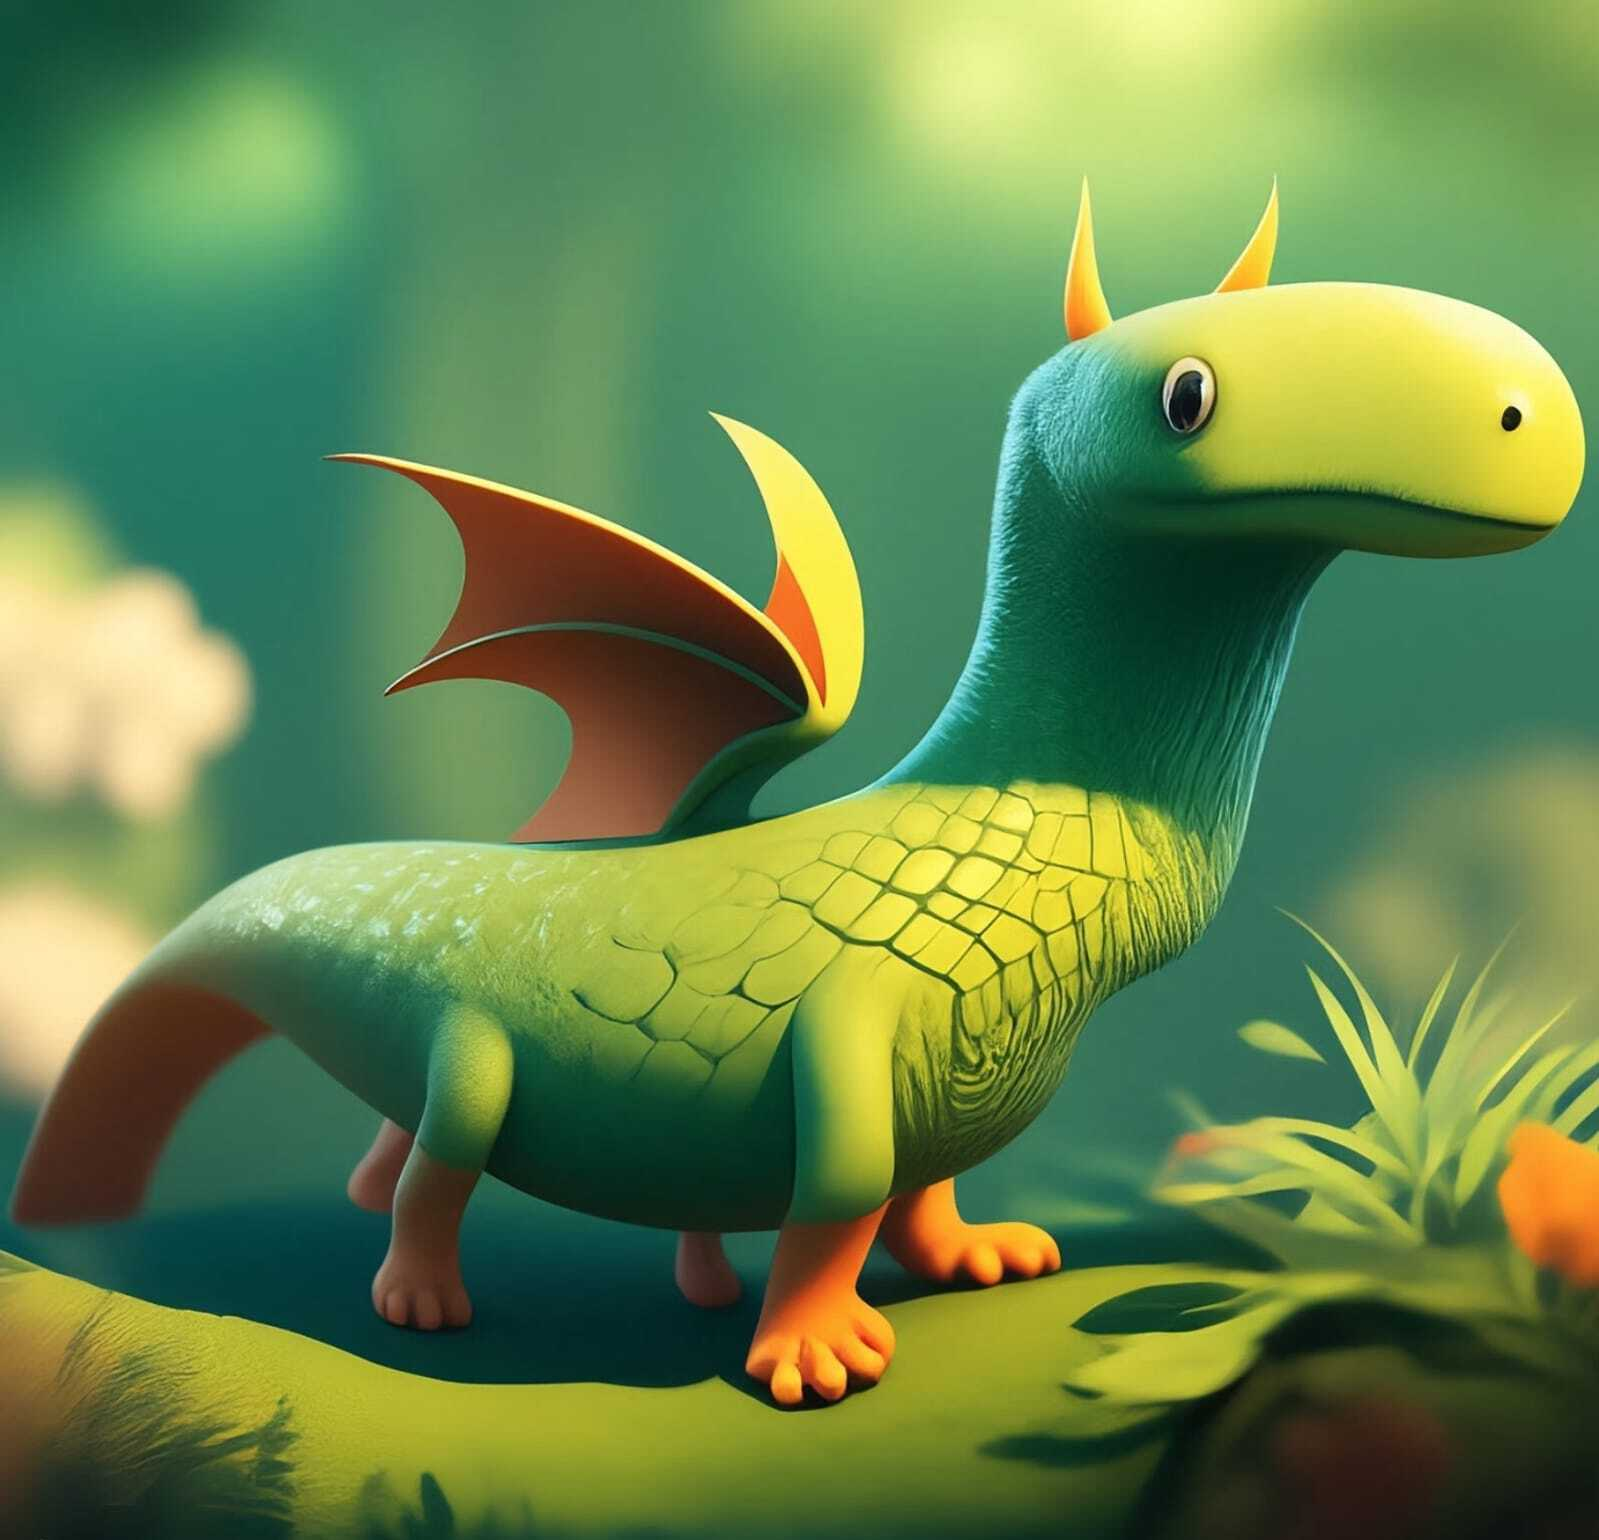
\includegraphics[width=6cm]{cover}
\end{center}
}

% theorem commands
\newtheoremstyle{c_remark}
	{}	% Space above
	{}	% Space below
	{}% Body font
	{}	% Indent amount
	{\bfseries}	% Theorem head font
	{}	% Punctuation after theorem head
	{.5em}	% Space after theorem head
	{\thmname{#1}\thmnumber{ #2}\thmnote{ \normalfont{\text{(#3)}}}}	% head content
\newtheoremstyle{c_definition}
	{3pt}	% Space above
	{3pt}	% Space below
	{}% Body font
	{}	% Indent amount
	{\bfseries}	% Theorem head font
	{}	% Punctuation after theorem head
	{.5em}	% Space after theorem head
	{\thmname{#1}\thmnumber{ #2}\thmnote{ \normalfont{\text{(#3)}}}}	% head content
\newtheoremstyle{c_plain}
	{3pt}	% Space above
	{3pt}	% Space below
	{\itshape}% Body font
	{}	% Indent amount
	{\bfseries}	% Theorem head font
	{}	% Punctuation after theorem head
	{.5em}	% Space after theorem head
	{\thmname{#1}\thmnumber{ #2}\thmnote{ \text{(#3)}}}	% head content

\ifcsname c@english\endcsname
	\theoremstyle{plain}
	\newtheorem{theorem}{Theorem}[section]
	\newtheorem{lemma}[theorem]{Lemma}
	\newtheorem{proposition}[theorem]{Proposition}
	\newtheorem*{proposition*}{Proposition}
	%\newtheorem{corollary}[theorem]{אין חלופה עברית}

	\theoremstyle{definition}
	\newtheorem{definition}[theorem]{Definition}
	\newtheorem*{definition*}{Definition}
	\newtheorem{example}{Example}[section]
	\newtheorem{exercise}{Exercise}[section]

	\theoremstyle{remark}
	\newtheorem*{remark}{Remark}
	\newtheorem*{solution}{Solution}
	\newtheorem{conclusion}[theorem]{Conclusion}
	\newtheorem{notation}[theorem]{Notation}
\else
	\theoremstyle{c_plain}
	\newtheorem{theorem}{משפט}[section]
	\newtheorem{lemma}[theorem]{למה}
	\newtheorem{proposition}[theorem]{טענה}
	\newtheorem*{proposition*}{טענה}
	%\newtheorem{corollary}[theorem]{אין חלופה עברית}

	\theoremstyle{c_definition}
	\newtheorem{definition}[theorem]{הגדרה}
	\newtheorem*{definition*}{הגדרה}
	\newtheorem{example}{דוגמה}[section]
	\newtheorem{exercise}{תרגיל}[section]

	\theoremstyle{c_remark}
	\newtheorem*{remark}{הערה}
	\newtheorem*{solution}{פתרון}
	\newtheorem{conclusion}[theorem]{מסקנה}
	\newtheorem{notation}[theorem]{סימון}
\fi

% Questions related commands
\newcounter{question}
\setcounter{question}{1}
\newcounter{sub_question}
\setcounter{sub_question}{1}

\ifcsname c@english\endcsname
	\newcommand{\question}[1][0]{
		\ifthenelse{#1 = 0}{}{\setcounter{question}{#1}}
		\section{Question \arabic{question}}
		\addtocounter{question}{1}
		\setcounter{sub_question}{1}
	}

	\newcommand{\subquestion}[1][0]{
		\ifthenelse{#1 = 0}{}{\setcounter{sub_question}{#1}}
		\subsection{Part \alph{sub_question}}
		\addtocounter{sub_question}{1}
	}
\else
	\newcommand{\question}[1][0]{
		\ifthenelse{#1 = 0}{}{\setcounter{question}{#1}}
		\section{שאלה \arabic{question}}
		\addtocounter{question}{1}
		\setcounter{sub_question}{1}
	}

	\newcommand{\subquestion}[1][0]{
		\ifthenelse{#1 = 0}{}{\setcounter{sub_question}{#1}}
		\subsection{סעיף \localecounter{letters.gershayim}{sub_question}}
		\addtocounter{sub_question}{1}
	}
\fi

% import lua and start of document
\directlua{common = require ('../common')}

\GetEnv{AUTHOR}

% headers
\author{\AUTHOR}
\date\today

\title{פתרון מטלה 02 --- תורת ההסתברות (1), 80420}

\begin{document}
\maketitle
\maketitleprint{}

\Question{}
בוחרים באקראי סדרה של $n$ מספרים $[m]$ עם חזרות. נגדיר $p_m$ את ההסתברות שבסדרה שבחרנו יש מופע של אותו מספר שלוש פעמים לפחות, נניח גם ש־$n(m) = o(m^{2/3})$, נוכיח כי $\lim_{n \to \infty} p_m = 0$.
\begin{proof}
	על־פי הנתון מתקיים $\Omega = {[m]}^n$, וכן נגדיר פונקציית הסבתרות נקודתית אחידה, דהינו $p(\omega) = \frac{1}{m^n}$. \\*
	יהי $A_i$ עבור $i \in [m]$ המאורע ש־$i$ מופיע לפחות שלוש פעמים, אז מתקיים
	\[
		|A_i| = m^n - \binom{n}{2} {(m - 1)}^{n - 2} - \binom{n}{1} {(m - 1)}^{n - 1} - {(m - 1)}^n
	\]
	וכן $|\Omega| = m^n$, ולכן גם $\PP_p(A_i) = \frac{|A_i|}{|\Omega|}$. \\*
	עוד נגדיר $A = \bigcup_{i \in [m]} A_i$ המאורע שיש לפחות שלושה ממספר לאיזשהו מספר, אז מחסם האיחוד
	\[
		p_m
		= \PP(A)
		= \PP(\bigcup_{i \in [m]} A_i)
		\le \sum_{i \in [m]} \PP(A_i)
		= m \cdot \frac{|A_1|}{|\Omega|}
	\]
	ולכן
	\begin{align*}
		p_m
		& \le m \cdot \frac{1}{m^n} \cdot (m^n - \binom{n}{2} {(m - 1)}^{n - 2} - \binom{n}{1} {(m - 1)}^{n - 1} - {(m - 1)}^n) \\
		& = m - \binom{n}{2} \frac{{(m - 1)}^{n - 2}}{m^{n - 1}} - n \frac{{(m - 1)}^{n - 1}}{m^{n - 1}} - \frac{{(m - 1)}^n}{m^{n - 1}}
	\end{align*}
	לבסוף נבחין כי $n(m) = o(m^{2/3})$ ולכן $n \to \infty$ גורר $m \to \infty$, לכן נבחן את
	\[
		0 \le \lim_{m \to \infty} p_m
		\le \lim_{m \to \infty} m - \frac{1}{2} n (n - 1) \frac{{(m - 1)}^{n - 2}}{m^{n - 1}} - n \frac{{(m - 1)}^{n - 1}}{m^{n - 1}} - \frac{{(m - 1)}^n}{m^{n - 1}}
		= 0
	\]
	ולכן גם $\lim_{n \to \infty} p_m = 0$.
\end{proof}

\Question{}
בכל בוקר ילד מקבל מהוריו סכום קבוע לקנות חטיף. בכל חטיף נמצאות אחת מ־22 האותיות של האלפבית העברי בהסתברות שווה, ועל הילד להרכיב את המילה ''קטר''. \\*
נגדיר את האותיות לפי מספרים עד 22, ונגדיר שרירותית את האותיות ''קטר'' להיות 1 עד 3.

\Subquestion{}
עבור $n \in \NN$ נחשב את ההסתברות שביום ה־$n$ לילד לא הייתה האות $a$ עבור $a \in [3]$.
\begin{solution}
	לכל יום $\Omega_d = [22]$ עם פונקציית הסתברות אחידה $p(n) = \frac{1}{22}$, בהתאם לאחר $n$ ימים נקבל $\Omega = \Omega_d^n$, ואנו מחפשים את המאורע $A = \{ \omega \in \Omega \mid a \notin \omega\}$.
	נקבל $|A| = 21^n$, באופן דומה נקבל גם $|\Omega| = 22^n$, לכן
	\[
		\PP(A) = \frac{|A|}{|\Omega|} = \frac{21^n}{22^n}
	\]
\end{solution}

\Subquestion{}
נחשב את ההסתברות שלאחר $n$ ימים הילד עדיין לא הצליח להרכיב את המילה הרצויה על־ידי שימוש בנוסחת הכלה והדחה.
\begin{solution}
	נגדיר $A, B, C$ המאורע שלילד אין את האותיות הראשונה השנייה והשלישית לאחר $n$ ימים, מהכלה והפרדה נקבל
	\[
		\PP(A \cup B \cup C) = \PP(A) + \PP(B) + \PP(C) - \PP(A \cap B) - \PP(A \cap C) - \PP(B \cap C) + \PP(A \cap B \cap C)
	\]
	נבחין כי אנו מחפשים באמת את אחד מהמצבים בהם לפחות אחת מן האותיות חסרה, זהו אכן האיחוד של המאורעות, לעומת זאת מטעמי הסתברות אחידה נוכל כי
	\[
		\PP(A \cup B \cup C) = 3\PP(A) - 3\PP(A \cap B) + \PP(A \cap B \cap C)
	\]
	מצאנו כי $\PP(A) = \frac{21^n}{22^n}$, ובאופן דומה גם נוכל להסיק $\PP(A \cap B) = \frac{20^n}{22^n}$ ואף $\PP(A \cap B \cap C) = \frac{19^n}{22^n}$ ולכן
	\[
		\PP(A \cup B \cup C)
		= 3 \frac{21^n}{22^n} - 3 \frac{20^n}{22^n} + \frac{19^n}{22^n}
		= \frac{3 \cdot 21^n - 3 \cdot 20^n + 19^n}{22^n}
	\]
\end{solution}

\Question{}
בכד $n \ge 2$ כדורים ומתוכם אחד בצבע לבן והאחרים שחורים, מוציאים ללא החזרה שני כדורים ובוחנים את צבעיהם.

\Subquestion{}
נגדיר מרחב הסתברות מתאים.
\begin{solution}
	נגדיר מרחב הסתברות דו־שלבי, נתחיל בהגדרת $\Omega_1 = \{ B, W \}$, נתון כי $p(B) = \frac{n - 1}{n}$ וכי $p(W) = \frac{1}{n}$. \\*
	נעבור לניסוי השני, עבורו מתקיים $\Omega_2 = \Omega_1$, ונגדיר את פונקציית ההסתברות הנקודתית $p_W, p_B$ על־ידי
	\[
		p_W(W) = 0, p_W(B) = 1,
		p_B(W) = \frac{1}{n - 1}, p_B(B) = \frac{n - 2}{n - 1}
	\]
	בהתאם להגדרת הניסוי, לבסוף נגדיר את מרחב הניסוי $(\Omega_1 \times \Omega_2, \mathcal{F}_{1, 2}, \PP_q)$ עבור $q(a, b) = p(a) \cdot p_a(b)$.
\end{solution}

\Subquestion{}
נתון כי ההסתברות להוציא את הכדור הלבן כפולה מההסתברות שלא להוציא אותו, נמצא את $n$.
\begin{solution}
	נבחין כי ההסתברות לא להוציא את הכדור הלבן היא ההסתברות להוציא שני כדורים שחורים $q(B, B) = p(B) \cdot p_B(B) = \frac{n - 1}{n} \cdot \frac{n - 2}{n - 1} = \frac{n - 2}{n}$. \\*
	עוד נבחין כי ההסתברות להוציא כדור לבן היא $\PP(\{ WB, BW, WW \}) = q(W, B) + q(B, W) + q(W, W) = \frac{1}{n} \cdot 1 + \frac{n - 1}{n} \cdot \frac{1}{n - 1} + 0 = \frac{2}{n}$. \\*
	בהתאם נתון גם כי $2 \frac{n - 2}{n} = \frac{2}{n}$, ולכן נובע $n = 3$.
\end{solution}

\Question{}
$2^n$ שחקניות שונות אבל זהות בכישוריהן משתתפות בטורניר שחמט באורך $n$, ונניח שבכל משחק יש מנצחת ומפסידה בלבד, בסיבוב הראשון משחקות $2^n$ שחקניות, בסיבוב השני $2^{n - 1}$ המנצחות וכן הלאה.

\Subquestion{}
עבור $k \in \NN$ זוגי תהי $\Omega_p(k)$ קבוצת האפשרויות לחלק $k$ איברים לזוגות, נחשב את $|\Omega_p(k)|$.
\begin{solution}
	השאלה שקולה למספר התמורות המורכבות ממחזורים זוגיים נפרדים, דהינו נבחר כל פעם 2 ויצור ציוות שלהם, תוך הורדת המספר בהתאם, אם נתחיל ב־$k$ ואפס אפשרויות, נקבל $k - 2$ ו־$\binom{k}{2}$. \\*
	בשלב השני נקבל $k - 4$ נשארו ו־$\binom{k}{2} \binom{k - 2}{2} = \frac{k!}{2^2 (k - 4)!}$, אם נמשיך תהליך זה נקבל $\frac{k!}{2^{k / 2}}$. \\*
	עתה נבחין כי בתהליך זה מצאנו את מספר הזוגות כשהזוגות מסודרים, לכן עלינו לבטל את ההבחנה בהם, נקבל זאת על־ידי
	\[
		|\Omega_p(k)| = \frac{k!}{(k / 2)! 2^{k / 2}}
	\]
\end{solution}

\Subquestion{}
נחשב את ההסתברות ששתי שחקניות נתונות יפגשו בסיבוב הראשון.
\begin{solution}
	למעשה אם נקבע את הזוג הנתון נקבל את $|A| = |\Omega_p(k - 2)|$, וכמובן $|\Omega| = |\Omega_n(k)|$, לכן
	\[
		\PP(A)
		= \frac{\frac{(k - 2)!}{((k - 2) / 2)! 2^{(k - 2) / 2}}}{\frac{k!}{(k / 2)! 2^{k / 2}}}
		= \frac{(k - 2)!}{k!} \cdot \frac{(k / 2)! 2^{k / 2}}{(k / 2 - 1)! 2^{k / 2 - 1}}
		= \frac{2 k / 2}{k(k - 1)}
		= \frac{1}{k - 1}
	\]
\end{solution}

\Subquestion{}
נסמן $\Omega(2^n, 2)$ עבור כל $k \in \NN$ את קבוצת כל האפשרויות לבחור זוג איברים ללא חשיבות לסדר וללא החזרה מתוך $2^n$, נחשב את $|\Omega(2^n, 2)|$
\begin{solution}
	נראה דוגמה, אם אנו מחפשים את $\{ a, b \} \in \Omega(2^n, 2)$, אז יתכן כי בבחירת איבר אחד ואז השני נקבל $a$ ואז $b$, או $b$ ואז $a$, בשל אי־ההחזרה נסיק כי תחילה יש $2^n$ אפשרויות, ואז $2^{n - 1}$, ולבסוף נחלק ב־$2$. \\*
	לכן נסיק $|\Omega(2^n, 2)| = \frac{1}{2} 2^n (2^n - 1) = \binom{2^n}{2}$.
\end{solution}

\Subquestion{}
נחשב את ההסתברות ששתי שחקניות נתונות תיפגשנה בסיבוב האחרון.
\begin{solution}
	נבחין כי עבור שחקנית נתונה להגיע לגמר הוא אכן הליך מורכב ואיטרטיבי, אבל בשל האחידות נסיק כי סיכוי זה זהה עבור כל שחקנית, דהינו גם הסיכוי להגיע לגמר, ללא התחשבות בשאר חלקי התרות, הוא סיכוי אחיד. \\*
	נסיק אם כן שההסתברות אחידה, ובהתאם להגדרת השאלה אנו מחפשים את הסיכוי שזוג ספציפי יגיע לגמר, דהינו זהו החישוב שעשינו בסעיף הקודם. \\*
	לכן גם נוכל להסיק כי אם $A = \{ \{a, b\} \}$ עבור שתי שחקניות קבועות $a, b$, אז $\PP(A) = \frac{|A|}{|\Omega(2^n, 2)|} = \frac{2}{2^n (2^n - 1)}$
\end{solution}

\Subquestion{}
נחשב את הסיכוי ששתי שחקניות נתונות תיפגשנה במקום ה־$1 \le k \le n$.
\begin{solution}
	נבחין כי בסיבוב האחרון משחק אחד, בלפני אחרון 2 וכן הלאה, כן מספר המשחקים בסיבוב ה־$k$ הוא $2^{n - k}$, ובסיבוב זה יש $2 \cdot 2^{n - k}$ שחקניות, ובהתאם $\Omega(2^{n - k + 1}, 2) = \binom{2^{n - k + 1}}{2}$. \\*
	מצאנו את הגודל של מרחב המדגם, ועתה נגדיר $A = \{ \omega \in \Omega \mid \{ a, b \} \in \omega \}$ המאורע ששתי שחקניות משחקות בו ספציפית. \\*
	זה כמובן שקול למספר הזוגות כאשר יש קיבוע לשני זוגות, דהינו $2^{n - k + 1} - 2$ שחקניות, לכן $|A| = |\Omega(2^{n - k + 1} - 2, 2)$, נקבל אפוא
	\[
		\PP_k(A) = \frac{|A|}{|\Omega|} = \frac{\binom{2^{n - k + 1} - 2}{2}}{\binom{2^{n - k + 1}}{2}}
	\]
\end{solution}

\Subquestion{}
נחשב את ההסתברות ששתי שחקניות נתונות נפגשו מתישהו בטורניר.
\begin{solution}
	נוכל להניח כי כל סיבוב הוא בלתי תלוי באחרים בשל ההסתברות האחידה, ולכן נוכל להסיק
	\[
		\PP(A) = \biguplus_{1 \le k \le n} \PP_k(A)
	\]
\end{solution}

\Question{}
בוחרים באקראי באופן אחיד אחת מהקוביות $D_4, D_6, D_8$ מטילים אותה ומדווחים איזו קוביה נבחרה ומה תוצאת ההטלה, באופן זה מתקבלת הסתברות $\PP$ על $\Omega = \Omega_1 \times \Omega_2$ כאשר $\Omega_1 = \{ 4, 6, 8 \}$ ו־$\Omega = [8]$.

\Subquestion{}
נכתוב מפורשות את הניסוי הדו־שלבי שמגדיר את $\PP$.
\begin{solution}
	נתון כי הסתברות הניסוי הראשון היא אחידה, לכן $p(\omega) = \frac{1}{|\Omega_1|} = \frac{1}{3}$. \\*
	עתה נגדיר את הניסוי השני.
	עבור $\omega_1 = 4$ נקבל
	\[
		p_4(\omega_2) = \begin{cases}
			\frac{1}{4} & 1 \le \omega_2 \le 4 \\
			0 & 4 < \omega_2
		\end{cases}
	\]
	באופן דומה עבור $\omega_1 = 6$ נקבל
	\[
		p_6(\omega_2) = \begin{cases}
			\frac{1}{6} & 1 \le \omega_2 \le 6 \\
			0 & 6 < \omega_2
		\end{cases}
	\]
	ועבור $\omega_1 = 8$ נקבל $p_8(\omega_2) = \frac{1}{8}$. \\*
	לבסוף נגדיר $q(\omega_1, \omega_2) = p(\omega_1) \cdot p_{\omega_1}(\omega_2)$, ובהתאם $\PP = \PP_q$.
\end{solution}

\Subquestion{}
עתה נגדיר את פונקציית ההסתברות במקרה ההפוך, כאשר $\Omega_1' = [8], \Omega_2' = \{4, 6, 8\}$ כך שההסתברות נשארת זהה עבור $\Omega_2' \times \Omega_1'$ זהה ל־$\PP$ בסעיף הקודם.
\begin{solution}
	נבחין כי אנו יכולים להסתכל על מקרה זה בשתי דרכים שונות. אנו יכולים להתייחס למספרים כבעלי סיכוי שווה ועל הקוביות המתאימות כבעלות התפלגות שונה, והפוך. מטעמי נוחות, נסתכל בצורה הראשונה,
	לכן נגדיר $p(\omega_1) = \frac{1}{8}$. \\*
	אם $7 \le \omega_1 \le 8$ אז $p_{\omega_1}(8) = 1$, ובהתאם $p_{\omega_1}(4) = p_{\omega_1}(6) = 0$.
	זאת שכן רק קוביה $D_8$ מאפשרת קבלת מספר מטווח זה. \\*
	נעבור עתה למקרה $5 \le \omega_1 \le 6$, במקרה זה עדיין $p_{\omega_1}(4) = 0$, אך עלינו למצוא את ההסתברות במקרה של $6, 8$. \\*
	לדוגמה בסעיף א' $p(6, 6) = \frac{1}{3} \cdot \frac{1}{6} = \frac{1}{18}$ ולכן $p(\omega_1) \cdot p_{\omega_1}(6) = \frac{1}{18}$, אז נקבל $p_{\omega_1}(6) = \frac{4}{9}$. \\*
	מהשלמה נקבל גם $p_{\omega_1}(8) = \frac{5}{9}$. \\*
	נעבור למקרה האחרון ונניח $1 \le \omega_1 \le 4$, עתה כל שלוש הקוביות אפשריות לקבלה, ולכן נבצע חישוב דומה לזה שעשינו זה עתה. \\*
	בסעיף א' מתקבל $p(4, 1) = \frac{1}{3} \cdot \frac{1}{4}$ ולכן בהתאם $p(\omega_1) \cdot p_{\omega_1}(4) = \frac{1}{12}$ ולכן $p_{\omega_1}(4) = \frac{2}{3}$. \\*
	בהתאם מסעיף א' מתקבל $p(6, 1) = \frac{1}{18}$ ולכן $p_{\omega_1}(6) = \frac{8}{18} = \frac{4}{9}$, באופן דומה $p_{\omega_1}(8) = \frac{1}{3}$. \\*
	כמובן הסכום צריך להיות 1 ולכן ננרמל אותו, נקבל כי אם נחלק את הערכים ב־$\frac{9}{13}$ הסכום יצא 1 ובהתאם נקבל פונקציית הסתברות.
\end{solution}

\Question{}
יהי $(\Omega, \PP)$ מרחב הסתברות בדיד, עבור $A, B \subseteq \Omega$ נגדיר $\tilde{\PP}(A \times B) = \PP(A \cap B)$.

\Subquestion{}
נוכיח כי אם $|\Omega| > 1$ אז קיימות תת־קבוצות של $\Omega \times \Omega$ שלא ניתנות להצגה בצורה של $A \times B$ עבור $A, B \subseteq \Omega$.
\begin{proof}
	נתון כי $|\Omega| > 1$ ולכן קיימים $\omega_1 \ne \omega_2 \in \Omega$, ונגדיר $C = \{ (\omega_1, \omega_2), (\omega_2, \omega_1) \}$ ולכן $C \subseteq \Omega \times \Omega$. \\*
	עתה נניח כי קיימים $A, B \subseteq \Omega$ כך ש־$A \times B = C$, ולכן נקבל $\omega_1, \omega_2 \in A$ ובאופן דומה $\omega_1, \omega_2 \in B$, אבל $(\omega_1, \omega_1) \notin C$. \\*
	קיבלנו אם כך סתירה לקיום של $A, B$ כאלה, דהינו לא קיימים כאלה כלל.
\end{proof}

\Subquestion{}
נוכיח כי ניתן להרחיב את ההגדרה של $\tilde{P}$ לכל תת־הקבוצות של $\Omega \times \Omega$ כך שהיא תהיה פונקציית הסתברות בדידה על $\Omega \times \Omega$.
\begin{proof}
	נגדיר $q : \Omega \times \Omega \to [0, 1]$ על־ידי
	\[
		q(\omega_1, \omega_2) = \begin{cases}
			p(\omega_1) & \omega_1 = \omega_2 \\
			0 & \omega_1 \ne \omega_2
		\end{cases}
	\]
	כאשר $p$ פונקציית הסבתרות נקודתית של $\Omega$ עצמו. \\*
	הפונקצייה אכן אי־שלילית ומתקיים
	\[
		\sum_{(\omega_1, \omega_2) \in \Omega \times \Omega} q(\omega_1, \omega_2)
		= (\sum_{(\omega_1, \omega_1) \in \Omega \times \Omega} q(\omega_1, \omega_1)) + (\sum_{\substack{(\omega_1, \omega_2) \in \Omega \times \Omega \\ \omega_1 \ne \omega_2}} q(\omega_1, \omega_2))
		= (\sum_{\omega_1 \in \Omega} p(\omega_1)) + (\sum_{\substack{(\omega_1, \omega_2) \in \Omega \times \Omega \\ \omega_1 \ne \omega_2}} 0)
		= 1
	\]
	ולכן $q$ אכן פונקציית הסתברות, ונבחן את $\PP_q$. \\*
	אם $A \times B \subseteq \Omega \times \Omega$ אז נקבל
	\[
		\PP_q(A \times B)
		= \sum_{\omega_1 \in A, \omega_2 \in B} q(\omega_1, \omega_2)
		= (\sum_{\substack{\omega_1 \in A, \omega_2 \in B \\ \omega_1 = \omega_2}} q(\omega_1, \omega_2)) + (\sum_{\substack{\omega_1 \in A, \omega_2 \in B \\ \omega_1 \ne \omega_2}} q(\omega_1, \omega_2))
		= \sum_{\omega \in A \cap B} p(\omega)
		= \tilde{\PP}(A \times B)
	\]
	ולכן מצאנו כי $\tilde{\PP} = \PP_q \upharpoonright \{ A \times B \mid A, B \subseteq \Omega \}$.
\end{proof}

\Subquestion{}
נמצא דוגמה שבה מרחב ההסתברות $(\Omega \times \Omega, \tilde{\PP})$ שונה ממרחב המכפלה של מרחב הסתברות בדיד.
\begin{solution}
	נגדיר $(\Omega, \PP_p)$ מרחב הסתברות הטלת מטבע, דהינו $\Omega = \{ 0, 1 \}$ וכן $p(\omega) = \frac{1}{|\Omega|}$. \\*
	נקבל אם כך ש־$\tilde{\PP}(1, 0) = \PP_p(\{ 1 \} \cap \{ 0 \}) = \PP_p(\emptyset) = 0$. \\*
	לעומת זאת, עבור $\PP_2$ פונקציית הסתברות למרחב המכפלה $\Omega \times \Omega$ נקבל $\PP_2(1, 0) = \frac{1}{|\Omega \times \Omega|} \ne 0$ שכן זהו מרחב הסתברות בדיד ואחיד. \\*
	שוני זה כמובן הוא מספיק כדי שמרחבי ההסתברות יהיו שונים.
\end{solution}


\end{document}
